\documentclass{article}
\usepackage[utf8]{inputenc}
\usepackage[margin=1in]{geometry}
\usepackage{amsmath, amsfonts}
\usepackage{fancyhdr}
\usepackage{multicol}
\usepackage{graphicx}
\usepackage[inline]{enumitem}
\usepackage{wrapfig}
\usepackage[export]{adjustbox}
\graphicspath{ {images/} }
\pagestyle{empty}
\fancyhf{}
\cfoot{\thepage}
\pagenumbering{gobble}

\lhead{MATB42: Assignment \#8}
\rhead{
Poon, Keegan\\
1002423727\\
Mar 20th 2018}
\newcommand{\norm}[1]{\| #1 \|}
\newcommand{\deriv}[1]{\frac{d}{d #1}}
\newcommand{\parti}[1]{\frac{\partial}{\partial #1}}
\renewcommand{\headrulewidth}{0pt}
\newcommand{\gam}{\boldsymbol{\gamma}}
\begin{document}

\thispagestyle{fancy}
\begin{enumerate}
    \begin{multicols}{2}
    \item A surface $S$ is obtained by rotation the given figure in the $xy$-plane about the $z$-axis. (The arc is part of a circle of radius 1 centered at (2,0).)
        \begin{enumerate}
            \item Paratemetrize $S$ (in pieces) and compute the surface area.

            We have that the upper line when rotated, can be parametrized by a restricted cone and similarly for the bottom. The top and bottom respectively can be written as 
        \end{enumerate}
            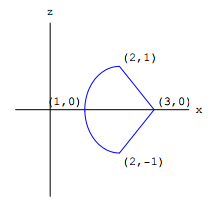
\includegraphics[width=0.25\textwidth]{b42-a8-q1ex}
    \end{multicols}
    \[ \boldsymbol \Phi_1 (u,\theta) = ((1-u)3 \cos \theta, (1-u)3 \sin \theta, 3u) ,\; 0\leq u \leq 1,\, 0 \leq \theta \leq 2\pi\] 
    \[ \boldsymbol \Phi_2 (u,\theta) = ((1+u)3 \cos \theta, (1+u)3 \sin \theta, -3u) ,\; -1 \leq u \leq 0 ,\, 0 \leq \theta \leq 2\pi\] 

    For the circular portion to the left, when rotated around, it will be the inner half of a torus, so the surface is
    \[ \boldsymbol \Phi_3 (\theta, \varphi) = ((2+\cos\varphi)\cos \theta, (2+\cos\varphi)\sin \theta, \sin \varphi)\]
    since it has radius 2 from the origin, and radius 1 from the center of the tube. Also $\theta \in [0,2\pi]$, but $\varphi$ restricted to $[\pi/2, 3\pi/2]$ for only the inner half.
    \[ \mathcal A (S) = \int_S \,dS = \int_{\boldsymbol \Phi_1} dS + \int_{\boldsymbol \Phi_2} dS + \int_{\boldsymbol \Phi_3} dS \]
    \begin{align*}
        &\boldsymbol \phi_{1_u} = (-3 \cos \theta, -3\sin \theta, 3) & &  \boldsymbol \phi_{1_ \theta} = (- (1-u) 3 \sin \theta, (1-u)3\cos\theta, 0) & \\
        & \boldsymbol \phi_{2_u} = (3 \cos \theta, 3\sin \theta, -3)  & & \boldsymbol \phi_{2_ \theta} = (- (1+u) 3 \sin \theta, (1+u)3\cos\theta, 0) & \\
        & \boldsymbol \phi_{3_\theta} = (-(2+\cos \varphi) \sin\theta, (2+\cos \varphi)\cos \theta, 0)  & & \boldsymbol \phi_{3_ \varphi} = (-\sin \varphi \cos \theta, -\sin \varphi \sin \theta, \cos \varphi) & \\
    \end{align*}
    \begin{align*}
        \boldsymbol \phi_{1_u} \times \boldsymbol \phi_{1_ \theta} &=       (-9(1-u)\cos\theta, -9(1-u)\sin\theta, -9(1-u)) \\
        \implies \norm {\boldsymbol \phi_{1_u} \times \boldsymbol \phi_{1_ \theta}} &= \sqrt{2(9^2(1-u)^2)} = \sqrt{2}(9(1-u)) \\
        \boldsymbol \phi_{2_u} \times \boldsymbol \phi_{2_ \theta} &=       (9(1+u)\cos\theta, 9(1+u)\sin\theta, 9(1+u)) \\
        \implies \norm {\boldsymbol \phi_{2_u} \times \boldsymbol \phi_{2_ \theta}} &= \sqrt{2(9^2(1+u)^2)} = \sqrt{2}(9(1+u)) \\
        \boldsymbol \phi_{3_\theta} \times \boldsymbol \phi_{3_ \varphi} &= (2 \cos\varphi \cos\theta + \cos\varphi^2 \cos\theta, 2 \cos \varphi \sin \theta + \cos^2 \varphi \sin \theta, \\
        & \; 2\sin \varphi \sin^2 \theta + \sin \varphi \cos \varphi \sin ^2 \theta + 2 \sin \varphi \cos^2 \theta + \sin\varphi \cos\varphi \cos^2 \theta ) \\
        &= (\cos\theta (2 \cos\varphi + \cos^2\varphi), \sin\theta (2 \cos \varphi + \cos^2 \varphi) , 2\sin \varphi + \sin \varphi \cos \varphi ) \\
        \implies \norm {\boldsymbol \phi_{3_ \theta} \times \boldsymbol \phi_{3_ \varphi}} &= \sqrt{(2\cos \varphi  + \cos^2\varphi)^2 + (2 \sin \varphi + \sin \varphi \cos \varphi)^2} \\
        &= \sqrt{(4\cos^2 \varphi  + 4 \cos^3 \varphi + \cos^4\varphi) + (4 \sin^2 \varphi + 4\sin \varphi^2 \cos\varphi + \sin^2 \varphi \cos^2 \varphi)} \\
        &= \sqrt{4 + 4 \cos^3 \varphi + \cos^4\varphi+  4\sin \varphi^2 \cos\varphi + \sin^2 \varphi \cos^2 \varphi} \\
        &= \sqrt{4 + 4 \cos^3 \varphi + \cos^2\varphi+  4\sin \varphi^2 \cos\varphi }\\
        &= \sqrt{4 + 4 \cos \varphi + \cos^2\varphi+ }\\
    \end{align*}

    (b) Use a computer algebra system to sketch $S$.

    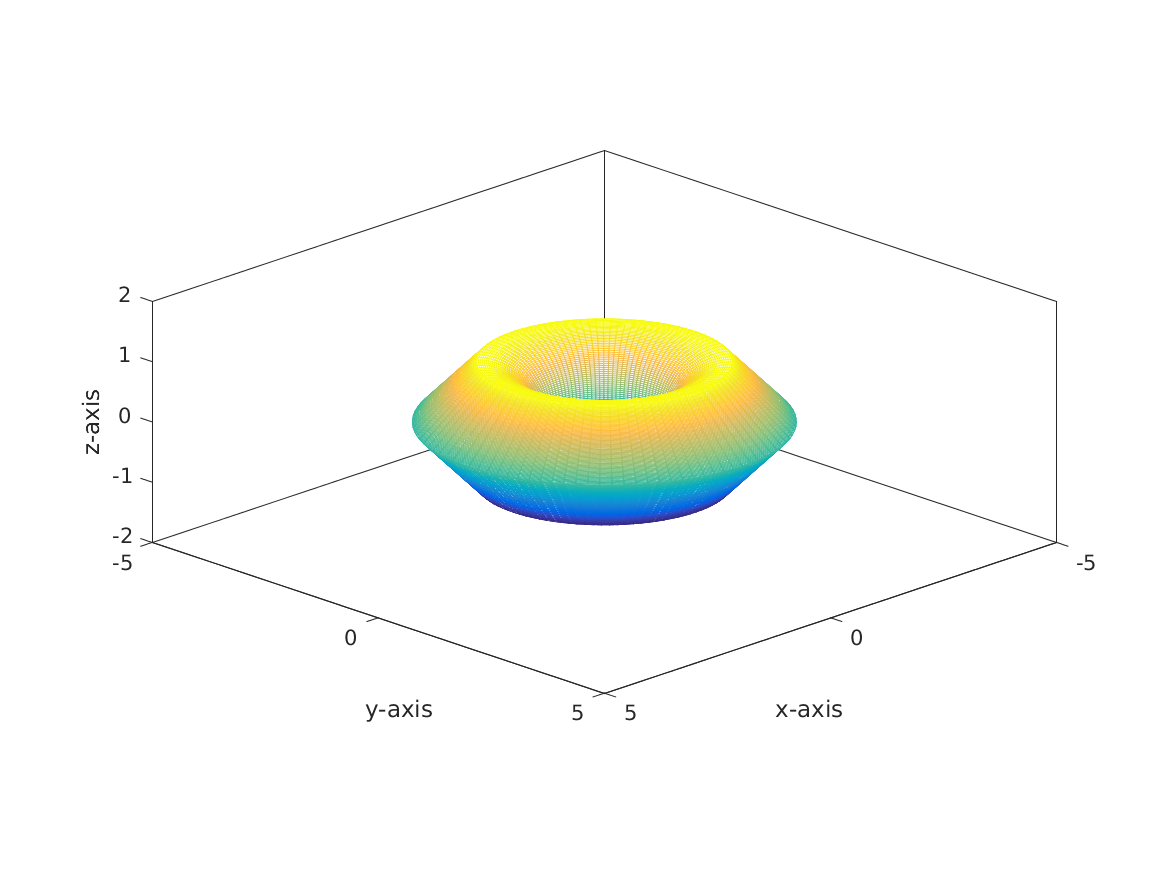
\includegraphics[width=0.7\textwidth,center]{b42-a8-1b}
    \newpage

    \item Let $S$ be the cone with vertex (2,3,3) and base the circle $x^2 + y^2 = 1$ in the $xy$-plane.
        \begin{enumerate}
            \item Paratemetrize $S$

            Starting with a base of a circle, we get $(\cos \theta, \sin \theta, 1)$ with $0 \leq \theta \leq 2\pi$. To change into a cone multiply $x$ and $y$ by $(1-u)$ with $0 \leq u \leq 1$ and finally to shift the vertex, add $(2u, 3u, 2u)$ where $z = 2u$ since the base equation already has a 1, so $1 + ku <= 3 \implies k \leq 2$.
            \[ \implies \boldsymbol \Phi (u,\theta) = ( (1-u)\cos \theta + 2 u, (1-u)\sin \theta + 3u, 1 + 2u) \] 
            \item Use a computer algebra system to sketch $S$.

                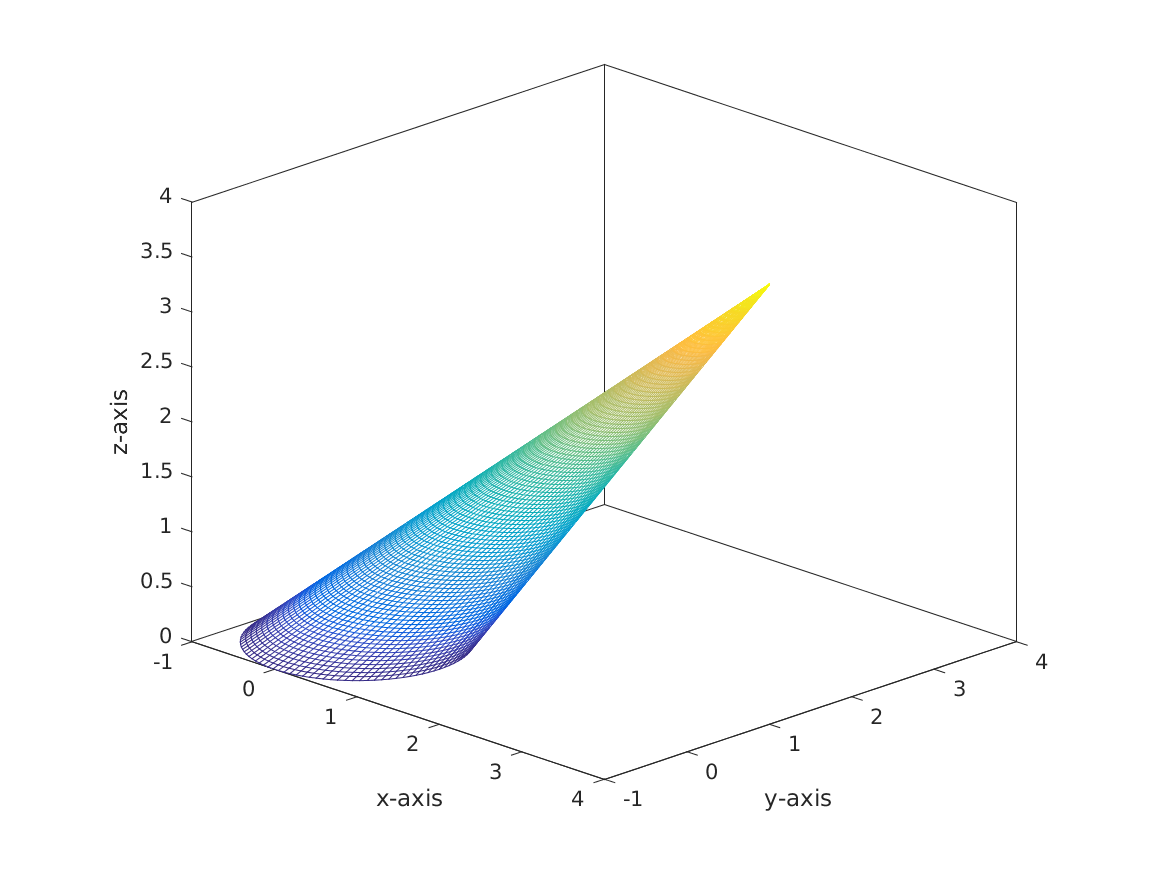
\includegraphics[width=0.7\textwidth,center]{b42-a8-2b}
            \item Write down the integral that would give the surface area of $S$. (You are not expected to evaluate the integral.)
            \begin{align*}
                \boldsymbol \phi_\theta &= (-(1-u)\sin \theta,\, (1-u)\cos \theta,\,0) \\
                \boldsymbol \phi_u &= (-\cos \theta + 2,\, -\sin\theta + 3,\,2) \\
                \boldsymbol \phi_\theta \times \boldsymbol \phi_u &= ((2(1-u)\cos \theta),  (2(1-u)\sin \theta),  \\ 
                & \; (-(1-u)\sin \theta)(-\sin \theta + 3) - ((1-u)\cos\theta)(-\cos \theta + 2)) \\
                &= ((2-2u)\cos \theta,  (2-2u)\sin \theta, (1-u)\sin^2 \theta -(3 - 3u)\sin \theta + (1-u)\cos ^2 \theta - (2-2u)\cos \theta) \\
                &= ((2-2u)\cos \theta,  (2-2u)\sin \theta, (1-u)-(3 - 3u)\sin \theta - (2-2u)\cos \theta) \\
                \norm{ \boldsymbol \phi_\theta \times \boldsymbol \phi_u} &= \sqrt{(2-2u)^2\cos^2 \theta +  (2-2u)^2\sin^2 \theta + ((1-u)-(3 - 3u)\sin \theta - (2-2u)\cos \theta)^2} \\
                &= \sqrt{(2-2u)+ ((1-u)-(3 - 3u)\sin \theta - (2-2u)\cos \theta)^2} \\
                \implies \mathcal{A}(S) &= \int_0^1\int_0^{2\pi} \sqrt{(2-2u)+ ((1-u)-(3 - 3u)\sin \theta - (2-2u)\cos \theta)^2}\, d\theta \, du \\
            \end{align*}
        \end{enumerate} 

    \newpage

    \item Let $S$ be the self-intersecting rectangle in $\mathbb{R}^3$ given by the implicit equation $x^2-y^2z=0.$
        \begin{enumerate}
            \item Give a parametrization of $S$ and use a computer algebra system to provide a sketch.

            \[x^2 - y^2z = 0 \implies y^2z = x^2 \implies z = \bigg(\frac{x}{y}\bigg)^2\]
            \[\boldsymbol \Phi (x,y) = \Bigg(x, y, \bigg(\frac{x}{y}\bigg)^2\Bigg)\]

            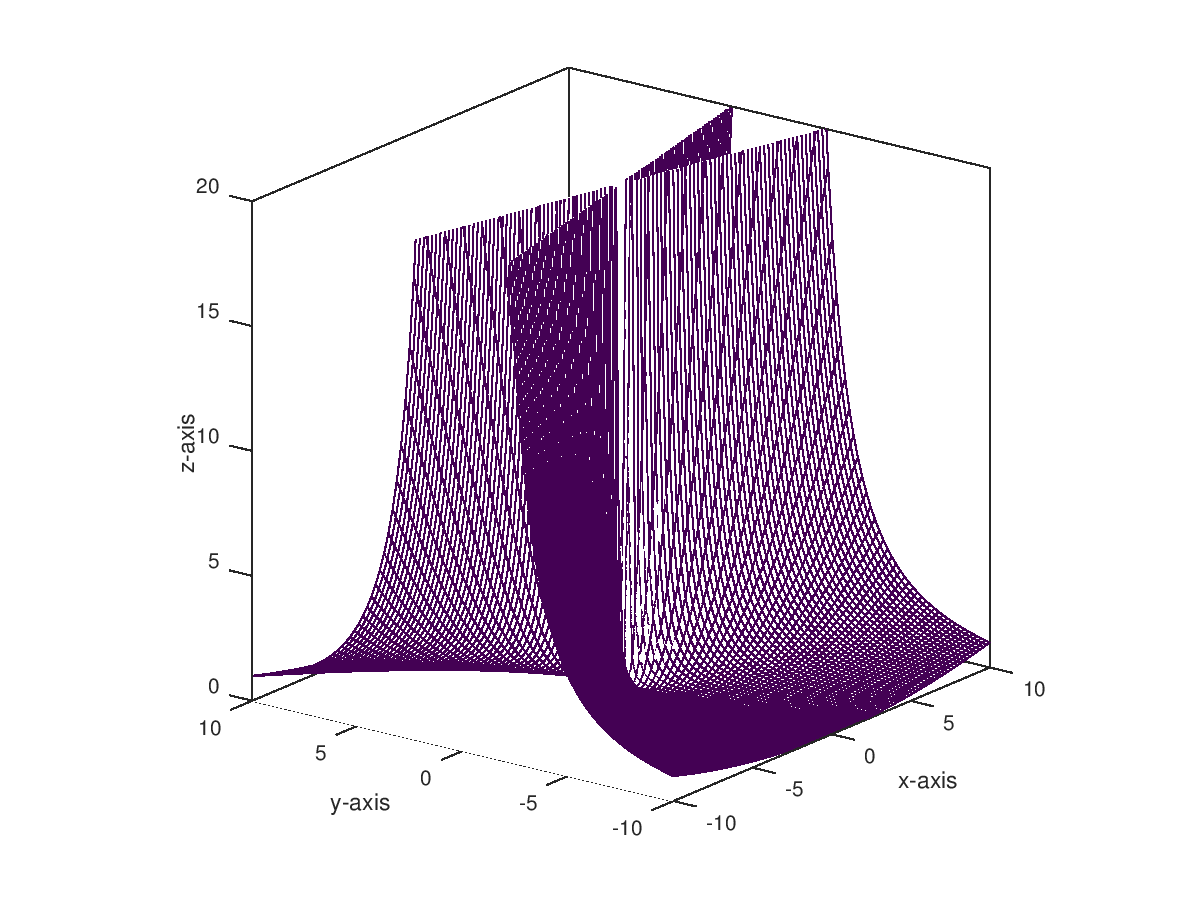
\includegraphics[width=0.75\textwidth,center]{b42-a8-3a}
            
            \item Is your parametrization one-to-one? Explain.

            Yes, if $\boldsymbol \Phi (x_0,y_0) = \boldsymbol \Phi (x_1,y_1)$ then $\Phi_1(x_0,y_0) = \Phi_2(x_1,y_1) \implies x_0 = x_1$, and $\Phi_2(x_0,y_0) = \Phi_2(x_1,y_1) \implies y_0 = y_1$. This means that $\boldsymbol \Phi (x_0, y_0) = \boldsymbol \Phi (x_1, y_1) \implies (x_0, y_0) = (x_1, y_1)$ so it is one to one.
            
            \item Find the equation of the tangent plane to $S$ at $\displaystyle \bigg( \frac{1}{4}, \frac{1}{2}, \frac{1}{4} \bigg).$

            \begin{align*}
                \boldsymbol \phi_x &= \bigg(1, 0, \frac{2x}{y^2}\bigg), \; \boldsymbol \phi_y = \bigg(0, 1, \frac{-2x^2}{y^3}\bigg) \\
                \boldsymbol \phi_x \times \phi_y &= \bigg(\frac{-2x}{y^2},\, \frac{2x^2}{y^3},\, 1\bigg) \\
                (\boldsymbol \phi_x \times \phi_y) \bigg(\frac{1}{4}, \frac{1}{2}\bigg) &= \bigg(\frac{-1/2}{1/4},\, \frac{1/8}{1/8},\, 1\bigg) \\
                &=(-2,1,1) \\
            \end{align*}
            So the tangent plane is defined by the equation \[ (-2)(x - 1/4) + (y - 1/2) + (z - 1/4) = 0 \Leftrightarrow-2x + y + z = 1/4 \]
        \end{enumerate}  
    \newpage 
    \item Let $S$ be the surface defined by $x^2 + y^2 = 1$ for $0 \leq z \leq 1$ and by $x^2 + y^2 = z^2$ for $1 \leq z \leq 2$.
        \begin{enumerate}
            \item Use symbolic algebra software to sketch $S$.

            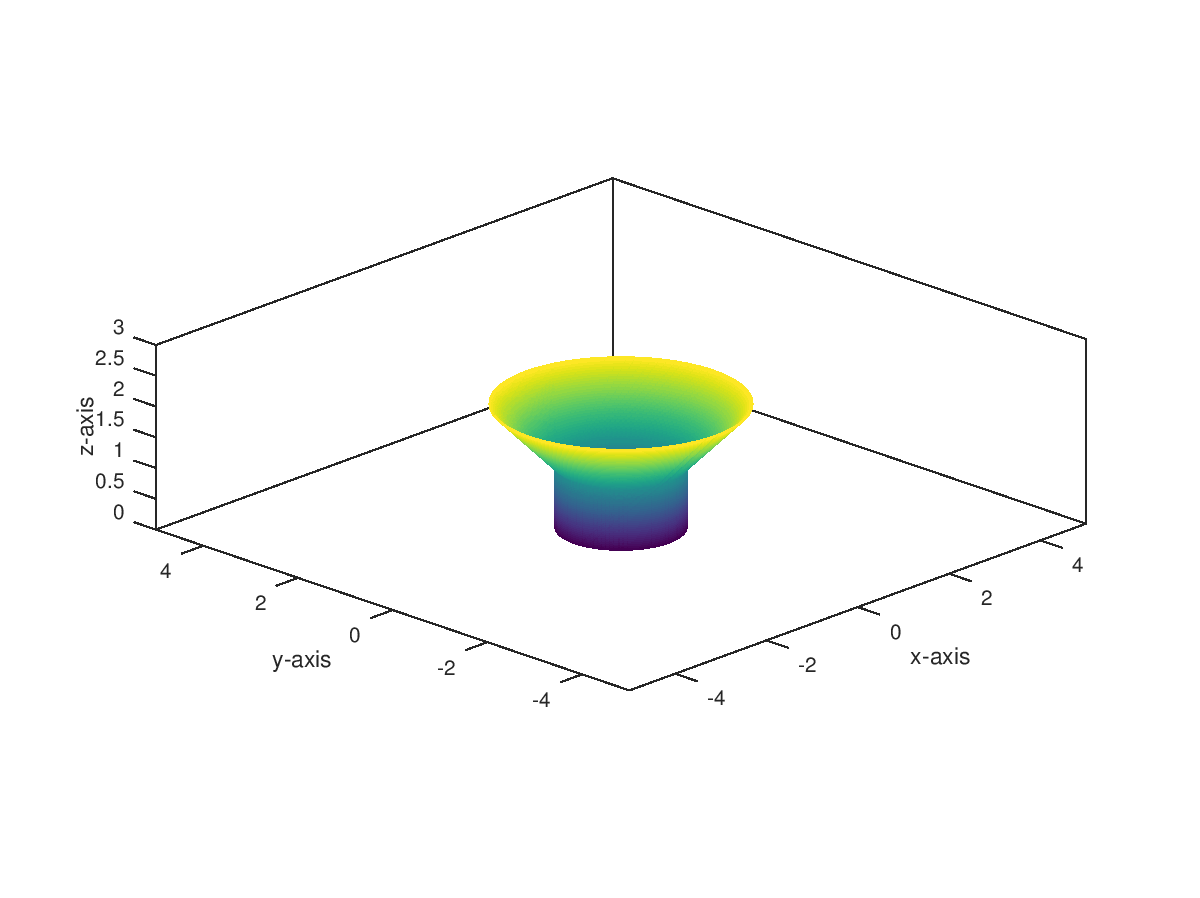
\includegraphics[width=0.5\textwidth,center]{b42-a8-4a}
            
            \item Evaluate $\displaystyle \int_S \boldsymbol F \cdot \, d \boldsymbol S $ where $\boldsymbol F (x,y,z) = (-y,x,z)$ and $S$ is oriented by outward pointing normals.

            $S$ can be parametrized piecewise by $\boldsymbol \Phi_1 (u, \theta) = (\cos \theta, \sin \theta, u)$ for $0 \leq u \leq 1$ and $\boldsymbol \Phi_2 (u, \theta) = (u\cos \theta, u\sin \theta, u)$ for $1 \leq u \leq 2$

            The derivatives of each are
            \begin{align*}
                \boldsymbol \phi_{1_u} &= (0,0,1)& &\boldsymbol \phi_{1_\theta} = (-\sin \theta,\cos \theta,0) \\
                \boldsymbol \phi_{2_u} &= (\cos \theta,\sin \theta,1)& &\boldsymbol  \phi_{2_\theta} = (-u\sin \theta,u\cos \theta,0) \\
            \end{align*}
            So their respective normals are 
            \begin{align*}
                &\boldsymbol  \phi_{1_u} \times \boldsymbol \phi_{1_\theta} = (-\cos \theta, -\sin \theta, 0)& &\boldsymbol  \phi_{2_u} \times \boldsymbol \phi_{2_\theta} = (-u\cos \theta, -u\sin \theta, u) & \\
            \end{align*}
            Examining the rightmost point (If projected into the $xy$-plane), where $\theta = 0$, both vectors will point towards the left  as $-\cos(0) = -1$ (since $u > 0$). These normals are orientation reversing, so their integrals will need to be of the opposite sign.

                \[\int_S \boldsymbol F \, d \boldsymbol S = \int_{\boldsymbol \Phi_1}\boldsymbol F(\boldsymbol \Phi_1) \cdot \, d \boldsymbol S + \int_{\boldsymbol \Phi_2} \boldsymbol F(\boldsymbol \Phi_2) \cdot \, d \boldsymbol S \]
            \begin{align*}
                \int_{\boldsymbol \Phi_1}\boldsymbol F(\boldsymbol \Phi_1) \cdot \, d \boldsymbol S &= - \int_0^1 \int_0^{2\pi} -(\sin\theta)(-\cos\theta) + (\cos\theta)(- \sin \theta) + (u)(0) \, d\theta \, du = 0 \\
                \int_{\boldsymbol \Phi_2} \boldsymbol F(\boldsymbol \Phi_2) \cdot \, d \boldsymbol S &= - \int_0^1 \int_0^{2\pi} -(u\sin\theta)(-u\cos\theta) + (u\cos\theta)(- u\sin \theta) + (u)(u) \, d\theta \, du  \\
                &= - \int_0^1 \int_0^{2\pi}  u^2 \, d\theta \, du = -\frac{2\pi}{3} \\
            \end{align*}
        \end{enumerate}  

    \newpage
    \item Evaluate the (vector) surface integral $\displaystyle \int_S \boldsymbol F \cdot \, d \boldsymbol S$ in each of the following cases.
        \begin{enumerate}
            \item $\boldsymbol F (x,y,z) = (1,x,z),\; S$ is the upper hemisphere $x^2+y^2+z^2 = 1,\, z \geq 0,$ with $\boldsymbol n $ pointing upward.
            
                A parametrization for $S$ is given by $\boldsymbol \Phi (\theta, \varphi) = (\cos\theta \sin\varphi, \sin\theta \sin\varphi, \cos\varphi)$, where $0 \leq \theta \leq 2\pi$ and $\displaystyle 0 \leq \varphi \leq \frac{\pi}{2}$
                \begin{align*}
                \boldsymbol \phi_{\theta} &= (- \sin \theta \sin \varphi, \cos \theta \sin \varphi, 0)\\
                \boldsymbol \phi_{\varphi} &= (\cos \theta \cos \varphi, \sin \theta \cos \varphi, -\sin \varphi) \\
                \boldsymbol \phi_\theta \times \boldsymbol \phi_\varphi &= (-\cos\theta \sin^2\varphi, -\sin\theta \sin^2\varphi, - \sin^2\theta \sin\varphi \cos\varphi - \cos^2\theta \sin \varphi \cos \varphi) \\ 
                &= (-\cos\theta \sin^2\varphi, -\sin\theta \sin^2\varphi, - \sin\varphi \cos\varphi ) \\ 
                \end{align*}
                Since $\sin\varphi, \cos\varphi \geq 0$ for $\varphi \in [0,\pi/2]$ this normal is orientation reversing, the sign needs to be flipped.
                \begin{align*}
                    \int_S \boldsymbol F \cdot \, d \boldsymbol S &= \int_0^{2\pi} \int_0^{\frac{\pi}{2}} (1,\cos\theta \sin\varphi,  \cos\varphi) \cdot (\cos\theta \sin^2\varphi, \sin\theta \sin^2\varphi,  \sin\varphi \cos\varphi ) \, d\varphi \, d\theta \\
                    &= \int_0^{2\pi} \int_0^{\frac{\pi}{2}}\cos\theta \sin^2\varphi + (\cos\theta \sin\varphi)(\sin\theta \sin^2\varphi)+  (\cos\varphi)(\sin\varphi\cos\varphi)) \, d\varphi \, d\theta \\
                    &=\int_0^{2\pi} \int_0^{\frac{\pi}{2}} \cos\theta \sin^2\varphi + \cos\theta \sin\theta \sin^3\varphi + \sin\varphi\cos^2\varphi \, d\varphi \, d\theta \\
                    &=\int_0^{2\pi} \int_0^{\frac{\pi}{2}} \cos\theta \sin^2\varphi + \frac{1}{2}\sin(2\theta)\sin^3\varphi \, d\varphi \, d\theta + \int_0^{2\pi} \int_0^{\frac{\pi}{2}}\sin\varphi\cos^2\varphi \, d\varphi \, d\theta \\
                    &=\int_0^{2\pi} \int_0^{\frac{\pi}{2}}\sin\varphi\cos^2\varphi \, d\varphi \, d\theta \; \text{[Integrate over full period of $\theta$]}\\
                    &\text{Let } u= \cos\varphi ,\, du = -\sin\varphi \\
                    &=\int_0^{2\pi} - \int_1^0 u^2\, d\varphi \, d\theta \\
                    &=2\pi \int_0^1 u^2\, d\varphi = \frac{2\pi}{3}\\
                \end{align*}
            \item $\boldsymbol F (x,y,z) = (2,x,z+y) ,\; S$ is that part of the plane $x+y+z = 1$ which lies in the first octant and $\boldsymbol n$ points upward.
                
                Parametrize $S$ as $\boldsymbol \Phi (x,y) = (x,y, 1-x-y)$ where $x \in [0,1],\, y \in [0, 1-x]$
                \[ \boldsymbol \phi_x = (1,0,-1) , \; \boldsymbol \phi_y = (0,1,-1),\; \boldsymbol \phi_x \times \boldsymbol \phi_y = (1,1,1)\]
                $z$ is positive for $\boldsymbol n$, so it is orientation preserving.
                \begin{align*}
                    \int_S \boldsymbol F \cdot \, d \boldsymbol S &= \int_0^1 \int_0^{1-x} (2,x, (1-x-y)+y) \cdot (1,1,1) \, dy \, dx \\
                    &= \int_0^1 \int_0^{1-x} 2+x+ 1-x \, dy \, dx = \int_0^1 \int_0^{1-x} 3 \, dy \, dx  \\
                    &= \int_0^1 3(1-x)\, dx = \int_0^1 3 - 3x \, dx  \\
                    &= 3 - \frac{3}{2} = \frac{3}{2} \\
                \end{align*}
                 \item Marsden \& Tromba, page 425, \#22.

                    Let $S$ be the part of the cone $z^2 = x^2 + y^2$ with $z$ between 1 and 2 oriented by the normal pointing out of the cone. Compute $\iint_S \boldsymbol F \cdot \, d \boldsymbol S$, where $\boldsymbol F (x,y,z) = (x^2, y^2, z^2)$.
                    
                    The parametrization for $S$ is given by $\boldsymbol \Phi (z, \theta) = (z\cos \theta, z\sin \theta, z),\, z \in [1,2],\, \theta \in [0,2\pi]$
                        \[ \boldsymbol \phi_z = (\cos \theta, \sin \theta, 1) , \; \boldsymbol \phi_\theta = (-z\sin\theta, z\cos\theta, 0),\; \boldsymbol \phi_z \times \boldsymbol \phi_\theta = (-z\cos\theta, -z\sin\theta, z) \]
                        Since $x, y$ are negative, the normal vector points inwards, this is an orientation reversing normal, so the sign needs to be flipped.
                        \begin{align*}
                            \int_S \boldsymbol F \cdot \, d \boldsymbol S &= - \int_0^{2\pi} \int_1^2 (z^2\cos^2\theta, z^2\sin^2\theta, z^2) \cdot (-z\cos\theta, -z\sin\theta, z) \, dz \, d\theta \\
                            &= \int_0^{2\pi} \int_1^2 z^3\cos^3\theta + z^3\sin^3\theta - z^3 \, dz \, d\theta \\
                            &= (16/4 - 1/4)\int_0^{2\pi} (\cos^3\theta + \sin^3\theta - 1) \, d\theta \\
                            &= \frac{15}{4} \bigg[ \int_0^{2\pi} \cos\theta(1 - \sin^2 \theta) \, d\theta + \int_0^{2\pi} \sin\theta(1 - \cos^2 \theta)\, d\theta + \int_0^{2\pi} - 1 \, d\theta \bigg] \\
                            &= \frac{15}{4} \bigg[ \int_0^{0} (1 - u^2 ) \, du - \int_1^{1} (1 - u^2 )\, du + \int_0^{2\pi} - 1 \, d\theta \bigg] \\
                            &= -\frac{15\pi}{2}
                        \end{align*} 
        \end{enumerate}

    \item Let $S$ be the portion of the plane $x-2y+z=1$ that is cut off by the coordinate planes and the plane $x+y=1$. Let $\boldsymbol V$ be the velocity field $\boldsymbol V (x,y,z) = (y,z,x^2)$. Find the flow across $S$ when $\boldsymbol n$ points upward. Explain your answer.

    \item Let $S$ be the closed surface that consists of the hemisphere $x^2+y^2+z^2 = 1,\, z \geq 0,$ and its base $x^2 + y^2 \leq 1,\, z = 0.$ let $\boldsymbol E$ be the electric field $\boldsymbol E(x,y,z) = (2x,2y,2z).$ Directly calculate the electric flux across $S$.
        
\end{enumerate}
\end{document}

